\chapter{Opdracht week 4}

\section{Toepassing 1}

Als eerste werdt er natuurlijk gedacht aan het originele idee,
een website waarop services gedeeld en ingehuurd worden.

\subsection{Relatie SWOT}
{\bf Hoe zijn we op dit idee gekomen, hoe is dit gerelateerd}

\subsection{Uitbreidingsplan}

\subsubsection{Doel}
{\bf Bedoeling met het systeem, welke partijen hebben er mee te maken}

\subsubsection{Impact}
{\bf Wat is er nodig, wat gebeurt er met het bedrijf}

Hieronder is een simpel voorbeeld van de onderliggende architectuur.

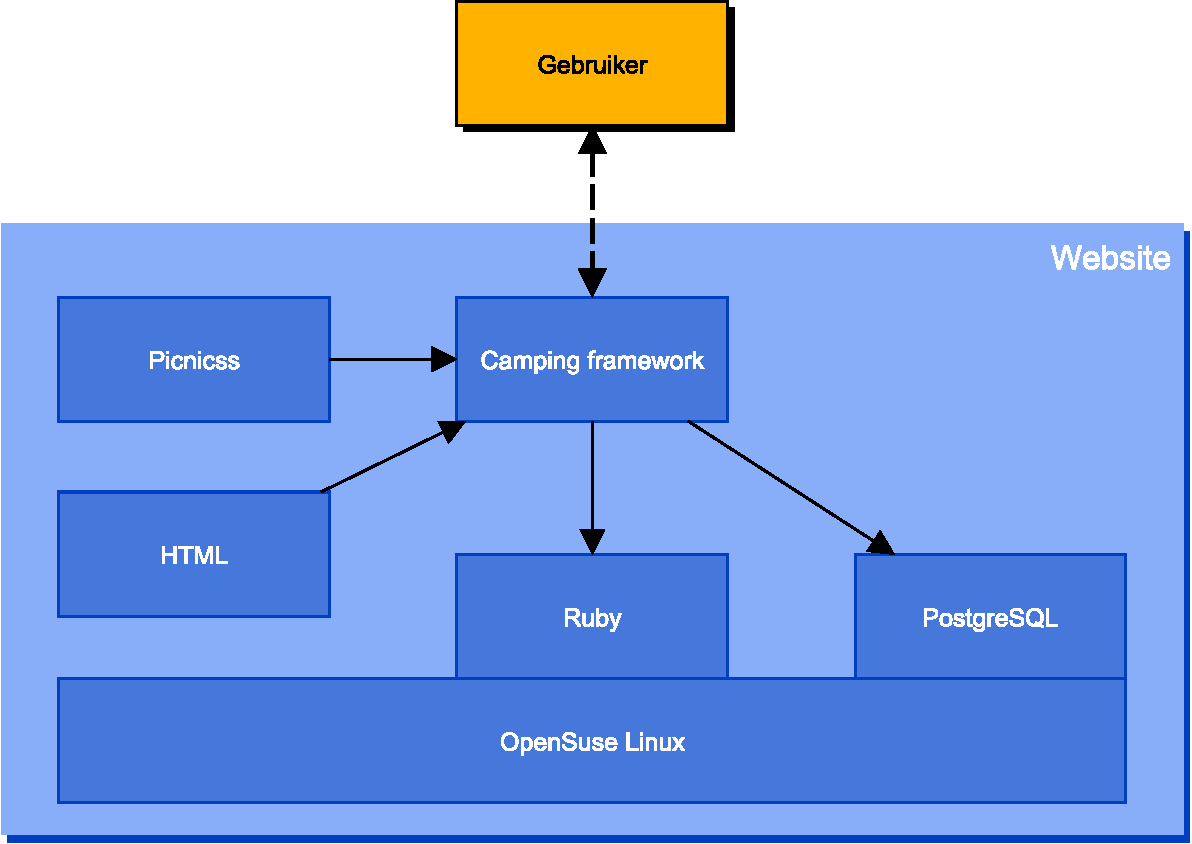
\includegraphics[width=\textwidth]{img/websiteArchitecture}

\subsubsection{Omschrijving}
{\bf Systeemontwerpen, wireframes, designs}

\section{Toepassing 2}

Een app zou eenzelfde soort functie kunnen leveren,
maar zal andere mensen aantrekken.
Een hypothese zou kunnen zijn dat een app het gemak verhoogd
en dus de markt groter maakt,
met een breder scala aan mensen.

\subsection{Relatie SWOT}
{\bf Hoe zijn we op dit idee gekomen, hoe is dit gerelateerd}

\subsection{Uitbreidingsplan}

\subsubsection{Doel}
{\bf Bedoeling met het systeem, welke partijen hebben er mee te maken}

\subsubsection{Impact}
{\bf Wat is er nodig, wat gebeurt er met het bedrijf}

\subsubsection{Omschrijving}
{\bf Systeemontwerpen, wireframes, designs}

\section{Toepassing 3}

Gezien we een handjevol competente ICT Beheerders in de groep hebben,
is het normaal om de benodigde ICT-gerelateerde services zelf te beheren.
Omdat er een grote kans is dat er meerdere servers benodigd zullen zijn,
is het belangrijk om een goede basis te hebben.

\subsection{Relatie SWOT}
{\bf Hoe zijn we op dit idee gekomen, hoe is dit gerelateerd}


\subsection{Uitbreidingsplan}

\subsubsection{Doel}
{\bf Bedoeling met het systeem, welke partijen hebben er mee te maken}

Dit systeem moet er voor zorgen dat het beheren van alle servers in het bedrijf
makkelijker en beter schaalbaar wordt door een deel ervan te automatiseren.

\subsubsection{Impact}
{\bf Wat is er nodig, wat gebeurt er met het bedrijf}

\subsubsection{Omschrijving}
{\bf Systeemontwerpen, wireframes, designs}
